\section{Design und Planung}

\subsection{Allgemeine Anforderungen}
In den Anfangsgesprächen wurden schon einige Anforderungen für die Planung festgelegt. 
Dabei wurde ein gemeinsamer Workspace in Notion erstellt, sowie ein gemeinsames Github-Repository.
Dadurch wurden für die Termine, sowie den Coding-Prozess eine \gls{ssot} gewährleistet.

Ebenso kamen die ersten Anforderungen der Entitäten zustande für das zukünftige \gls{erd}.

Das Hauptanwendungsszenario der Arbeit wurde definiert als \emph{Ein Nutzer kann Exhibitions erstellen und sich die Exhibitions von anderen Nutzern ansehen.} 
Alle weiteren Diskussionen über die Umsetzung dieses wurden anschließend in einem \gls{erd} zusammengefasst.

%\subsection{Erstellung eines Workspaces in Notion}
\subsection{Erstellung des ERDs}
Um zu gewährleisten, dass die Systemanforderung getroffen werden, ist es notwendig ein entsprechendes \gls{erd} zu erstellen.
Innerhalb eines \gls{erd} werden alle Entitäten, Attribute, sowie deren Beziehungen dargestellt.
Es dient als gemeinsamer Nenner für die Projektentwicklung, da jedes Teammitglied eine eigene Vorstellung der Datenstruktur haben könnte. 
Ein weiterer Vorteil eines \gls{erd}s ist das Potenzial Fehlerquellen zu identifizieren und dadurch zukünfige Problem zu umgehen. 

Nachdem die benötigten Entitäten, sowie deren Attribute festgelegt wurden, müssen nun die Beziehungen zueinander festgelegt werden. 
Dabei wird gewählt zwischen One-to-One, One-to-Many und Many-to-Many Beziehungen, wobei die Many-to-Many Beziehung innerhalb einer Assoziationstabelle dargestellt wird. 

Innerhalb dieser Arbeit ist die Entität \emph{Exhibitions} das zentrale Objekt, was in der Abbildung \ref{fig:erd:lastversion} gut ersichtlich ist.
Die Beziehungen zwischen \emph{Positionen, Exhibits, Rooms und Exhibitions} stellten sich besonders als Herausforderung dar, aufgrund der vielen Abhängigkeiten zueinander. 
Diese wurden besonders erst in der Implementierung ersichtlich, wodurch das \gls{erd} im Laufe der Entwicklung etwas angepasst wurde. 
Weitere Gründe für die Abänderung, waren Planänderungen bei der Kommunikation zwischen zwei Entitäten, sowie der Aufbau der Hauptentitäten \emph{Exhibition und Exhibit}. 
Die Unterschiede zwischen der ersten Version und der finalen sind deutlich (siehe Abb. \ref{fig:erd:firstversion} und \ref{fig:erd:lastversion}).
Besonders lassen sich die oben erläuterten Änderungen erkennen. 
 
\begin{figure}
    \centering
    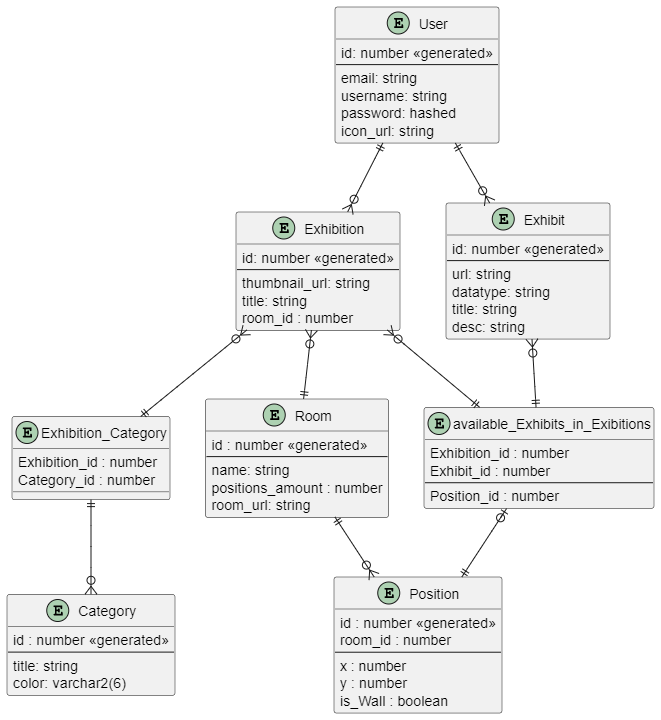
\includegraphics[scale=0.5]{pics/firstversion_erd.png}
    \caption{Erste Version des ERDs}
    \label{fig:erd:firstversion}
\end{figure}

\begin{figure}
    \centering
    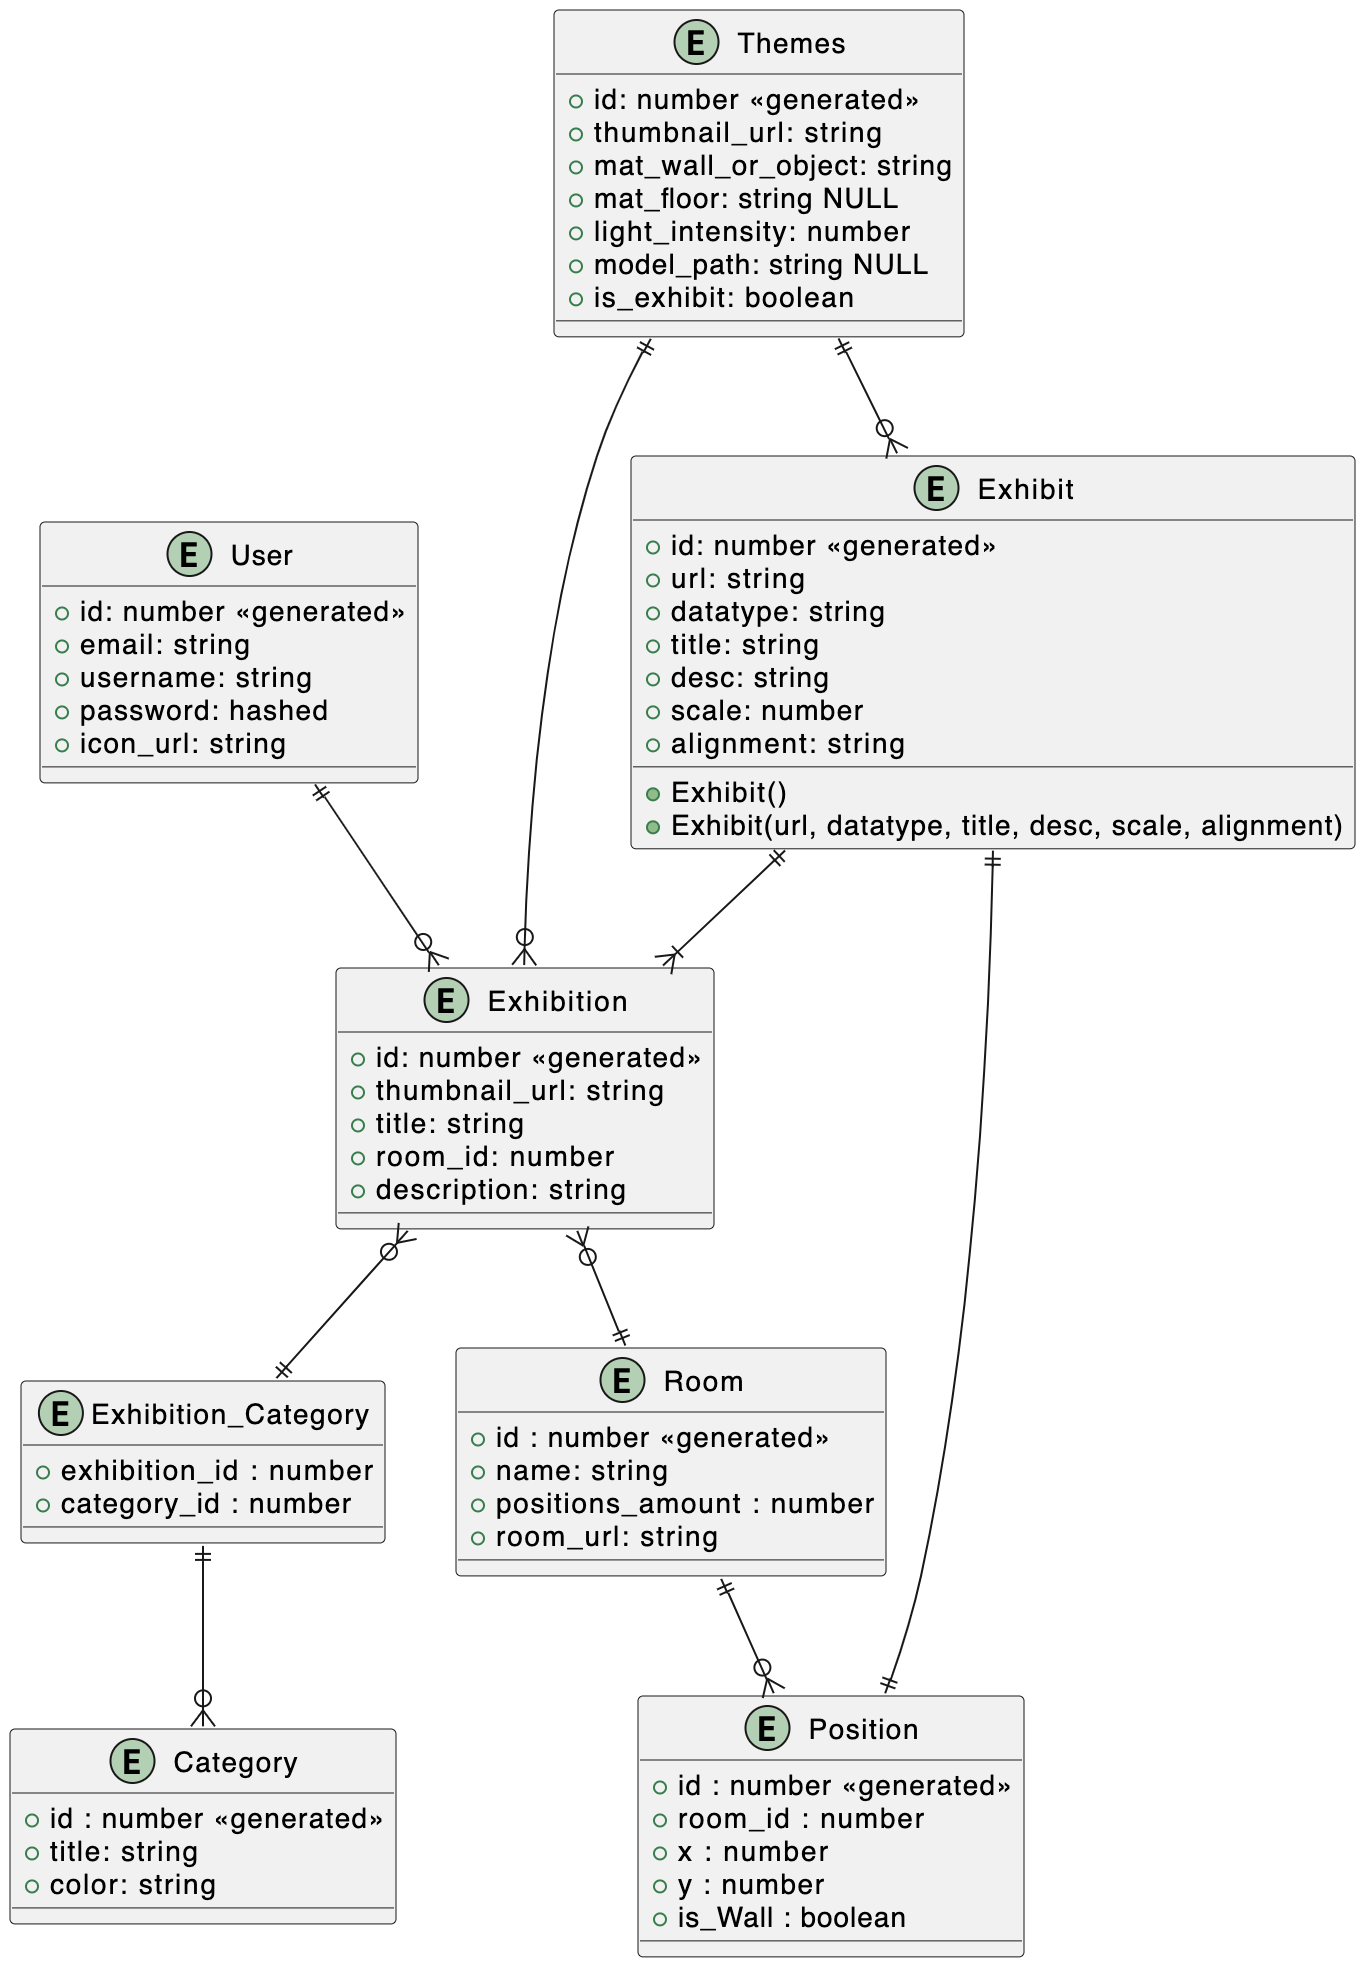
\includegraphics[scale=0.5]{pics/lastversion_erd.png}
    \caption{Finale Version des ERDs}
    \label{fig:erd:lastversion}
\end{figure}


\section{Aufsetzen der Datenbank und des Servers}

Um das Quarkus-Projekt aufzusetzen, gibt es mehrere Möglichkeiten. 
Online gibt es die Möglichkeit unter \href{https://code.quarkus.io}{code.quarkus.io} alle gewünschten Extensions mit Mausklick auszuwählen und anschließend das generierte Projekt herunterzuladen. 
Am Terminal besteht die Optionen mittels Maven oder Quarkus-\gls{cli}-Befehl ein Projekt zu erstellen, wobei gewünschte Erweiterungen händisch eingetippt werden müssen.

\begin{figure}
    \centering
    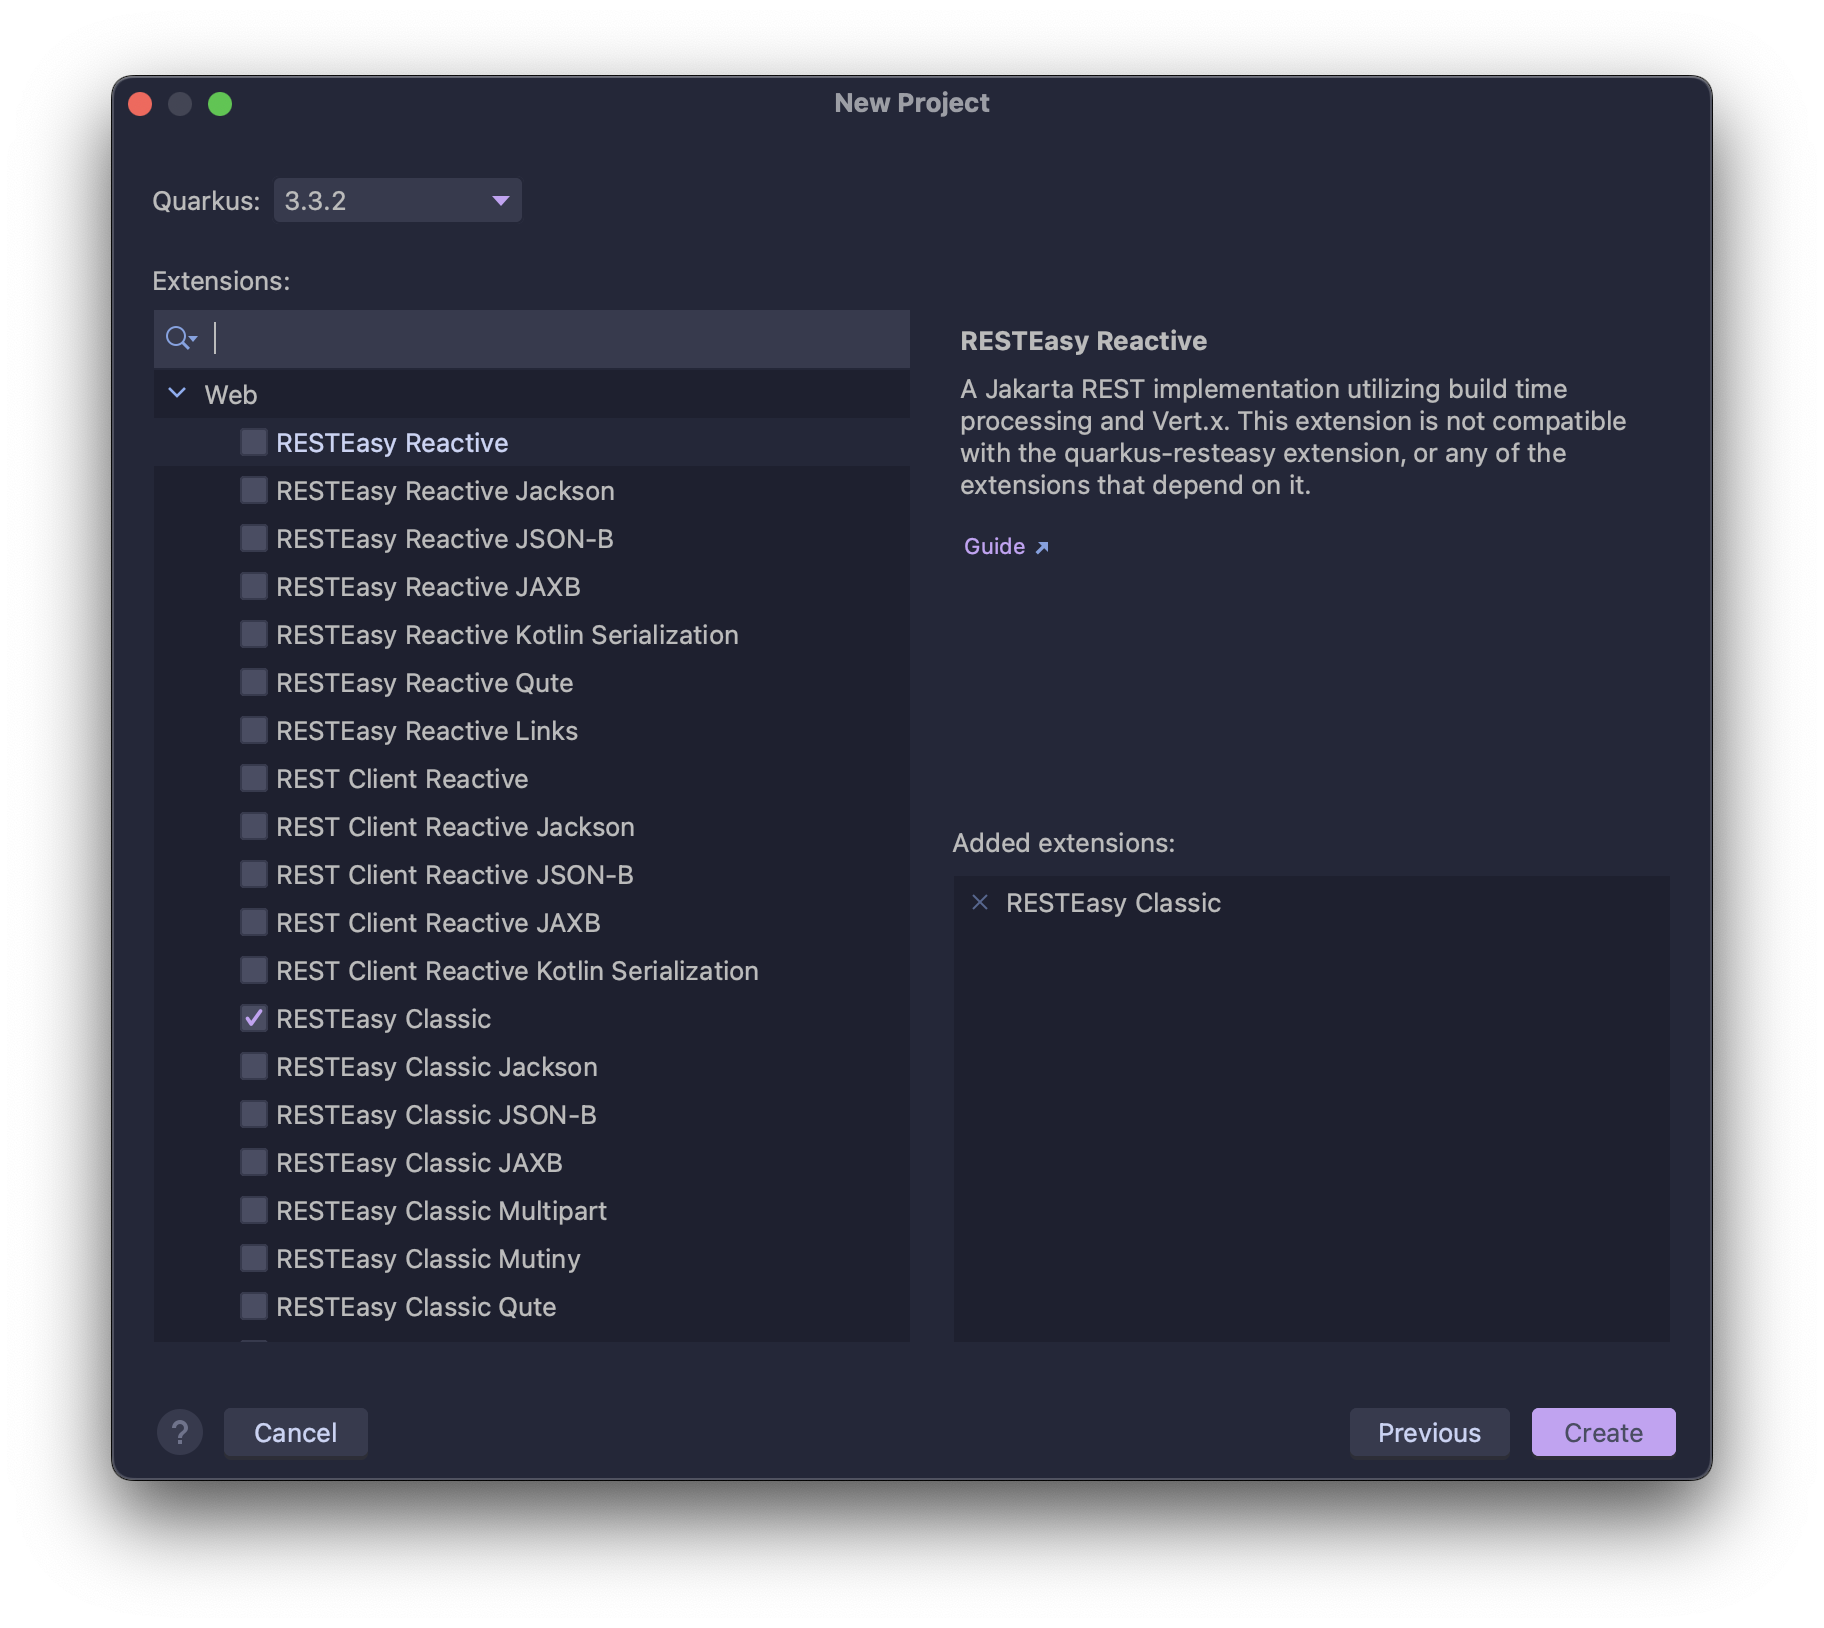
\includegraphics[scale=0.35]{pics/quarkusplugin.png}
    \caption{Auswählen der gewünschten Quarkus Extensions im Quarkus Plugin}
    \label{fig:intellij:plugin}
\end{figure}

Für diese Arbeit wurde jedoch das IntelliJ Plug-In \emph{Quarkus} von JetBrains s.r.o. verwendet. 
Dieses bildet dieselben Möglichkeiten, wie die Webseite, in einem griffbereitem \gls{ide}-Fenster ab (siehe Abb. \ref{fig:intellij:plugin}).
Dadurch muss kein weiteres Programm, wie ein Browser, gestartet werden nur für die Projekterstellung.
Zusätzlich werden Tools zur Verfügung gestellt, wie zum Beispiel Code-Assistenz, oder Laufkonfigurationen. \cite{QuarkusPlugin}

Durch die Verwendung von Maven werden alle Extensions im \emph{pom.xml}-File des Projekts gespeichert. 
Falls Erweiterungen im Nachhinein noch hinzugefügt werden sollen, kann dies durch Terminal Befehle automatisch geschehen, oder durch manuelles Einfügen in die Datei. 
Bei letzterem muss in den meisten Fällen ebenso die Maven manuell neu geladen werden, da Änderungen sonst nicht übernommen sein könnten. 

\begin{lstlisting}[label=lst:quarkus:mvnextension, language=xml, caption=Quarkus-\gls{cli}-Befehl für RESTEasy Classic]
    quarkus ext add io.quarkus:quarkus-resteasy
\end{lstlisting}

\begin{lstlisting}[label=lst:quarkus:mvnextension, language=xml, caption=Extension RESTEasy Classic in pom.xml]
<dependency>
    <groupId>io.quarkus</groupId>
    <artifactId>quarkus-resteasy</artifactId>
</dependency>
\end{lstlisting}

Nach der Erstellung des Projektes, sollte es sofort ausgeführt werden, um sicherzustellen, dass es keine fundamentalen Probleme am Projekt gibt. 
Dazu wird das \emph{developer} Profil von Quarkus genutzt, was mehr Funktionen ermöglicht, wie zum Beispiel das Loggen der Konsole.
IntelliJ konfiguriert die den Befehl automatisch, sodass dafür nur ein Buttonklick zuständig ist. 
Alternativ kann auch das Terminal verwendet werden. 
\begin{lstlisting}[label=lst:quarkus:devrun, language=bash, caption=Quarkus-\gls{cli}-Befehl zum Starten]
quarkus dev
\end{lstlisting}
 
Da mit der Anwendung Tabellen erstellt werden sollen, wird eine Datenbankverbindung benötigt. 
Dazu wird PostgreSQL am Gerät installiert und gestartet. 
\begin{lstlisting}[label=lst:quarkus:devrun, language=bash, caption=Homebrew Installation und Ausführung PostgreSQL]
brew install postgres
brew services start postgres
\end{lstlisting}

Als nächsten Schritt wird eine Verbindung von der Quarkus Applikation zu PostgreSQL aufgebaut. 
Name, Rolle bzw. User und Port der Datenbank können frei konfiguriert werden, allerdings wurden hier die standardmäßig definierten Werte gelassen. 
Für den Verbindungsaufbau während der Entwicklung werden die Einstellungen in Abbildung \ref{lst:quarkusDatasourceProject} genutzt. 
Falls die Anwendung auf eine Cloud hochgeladen wird, müssen andere Parameter gesetzt werden.

\begin{lstlisting}[label=lst:quarkusDatasourceProject, caption=Datenbankkonfiguration in \emph{application.properties}]
quarkus.datasource.db-kind=postgresql
quarkus.datasource.username = postgres
quarkus.datasource.password = postgres
quarkus.datasource.jdbc.url=jdbc:postgresql://localhost:5432/postgres

quarkus.hibernate-orm.database.generation=drop-and-create
\end{lstlisting}

Nachdem die Einstellungen eingefügt wurden, muss die Anwendung neu gestartet werden. 
Falls der Verbindungsaufbau versagt, wirft Quarkus während der Kompilierung Fehlermeldungen. 
Andernfalls können nun die Tabellen angelegt werden. 

\subsection{Umsetzung des ERDs in Quarkus}
Für den nächsten Schritt wird die Extension \emph{Hibernate ORM mit Panache} verwendet.
Mittels dieser werden Tabellen durch Definition der Annotation \emph{@Entity} erstellt. 
Die Annotation sieht vor, dass in jeder Entity-Klasse eine Id steht.
Durch die Ableitung der \emph{PanacheEntity}-Klasse (siehe Abb. \ref{lst:exhibitionEntityCode}, Zeile2), die schon eine Id in sich trägt, muss sie nicht mehr explizit definiert werden. 
Diese Id wurde ebenso als Primärschlüssel genutzt, da sie durch Generierung immer einzigartig ist.

In der Klasse werden alle Attribute als Variablen, gemäß des \gls{erd}s definiert. 
Die Beziehungen werden durch die Annotationen \emph{@OneToMany, @ManyToMany und @OnetoOne} über der dazugehörigen Variable dargestellt. 
Auf der gegenseitigen Entität muss ebenso eine Variable erstellt werden, wobei da die Annotation etwas anders aussieht. 
Diese muss die \emph{mappedBy}-Einstellung konfigurieren, da ansonsten die Beziehung mehrmals generiert wird (siehe Abb. \ref{lst:exhibitionEntityCode}, Zeile 4). 
Bei Many-to-Many wird zusätzlich die Annotation @JoinTable hinzugefügt, um die Assoziationstabelle zu konfigurieren (siehe Abb. \ref{lst:exhibitionEntityCode}, Zeilen 5 bis 12). 
Zu den Relationen können zusätzlich noch Cascade Types festgelegt werden. 
Dessen Funktionen werden in Unterkapitel \nameref{chap:cascade} genauer erklärt. 

\begin{lstlisting}[label=lst:exhibitionEntityCode, language=java, caption=Teil der Exhibition Entität]
@Entity
public class Exhibition extends PanacheEntity {
    // ...
    @OneToMany(mappedBy = "exhibition", cascade = CascadeType.REMOVE)
    public List<Exhibit> exhibits;

    @ManyToMany
    @JoinTable(
            name = "exhibitions_categories",
            joinColumns = @JoinColumn(name = "exhibition_id"),
            inverseJoinColumns = @JoinColumn(name = "category_id")
    )
    public Set<Category> categories;
}
\end{lstlisting}

Nachdem die Klassen komplett sind, muss die Anwendung neu gestartet werden. 
In den \emph{application.properties} wurde durch \emph{drop-and-create} konfiguriert, dass alle Tabellen bei Neustart gelöscht und neu aufgesetzt werden. 
Diese Einstellung sorgt dafür, dass die Änderungen tatsächlich übernommen werden. 

Ebenso wird bei jedem Start eine \emph{import.sql}-Datei aufgerufen, die vordefinierten Daten bei jedem Start automatisch in die Datenbank lädt.  
Für die Entitäten Theme, Positionen und Rooms hat sich das Team dazu entschieden, diese vorzugeben. 
Andere Entitäten werden als Testdaten in das File eingefügt und besitzen negative Ids. 
Die negativen Werte stellen sicher, dass keine Objekte in die Datenbank geladen werden, mit demselben Primärschlüssel.

\begin{lstlisting}[label=lst:importsql, language=sql, caption=Ausschnitt import.sql]
insert into category(id, category_title, color) values (1, 'Umwelt', '#C1BAFF'), (2, 'Tiere', '#ADD0FF');
insert into exhibit(id, title, description, scale, alignment, url, exhibition_id, position_id, data_type) values (-20, 'Art Blob', 'Sculpture made by Lorenz Litzlanze', 40, 'c', 'example-exhibits/abstraktArtBlob.gltf', -3, 2, 'gltf');
\end{lstlisting}

\subsubsection{User}
Die Entität eines Nutzenden, wird User genannt, wobei für den Tabellennamen in der Datenbank jedoch eine alternative Bezeichnung definiert ist.
Grund dafür ist, dass der Name \emph{User} in PostgreSQL reserviert ist. 
Deshalb ist in Codeausschnitt \ref{lst:userentity} die Zeile 2 erforderlich.

Ein neuer User muss nur ein Nutzername und ein Passwort besitzen.
Eine Id wird, wie vorhin erwähnt, automatisch generiert. 
Mittels der Attribute der \emph{@Column} Annotation, lassen sich obligatorische Felder definieren.
Ebenso können Feldlänge, Spaltenname und vieles mehr auf diese Art konfiguriert werden.

\begin{lstlisting}[label=lst:userentity, language=Java, caption=Teil der Entity-Klasse des Users]
@Entity
@Table(name="Users")        
public class User extends PanacheEntity {
    @Column(nullable = false, length = 50)
    public String user_name;
    @Column(nullable = false)
    public String password;
    public String email;
    //...
}
\end{lstlisting}

\subsubsection{Cascade Types}
\label{chap:cascade}

Cascade Types werden für Datenkonsistenz benötigt, da manche Objekte von anderen abhängen. 
Die verschiedenen Types entscheiden, was bei der Änderung eines Teils der Abhängigkeit passiert. 
Es gibt verschiedene Arten von Cascade Typen, dieser Arbeit hauptsächlich die unten aufgelisteten verwendet wurden.
\cite{CascadeTypes}

\begin{compactitem}
    \item \textbf{CascadeType.ALL}: Alle Operationen werden auf die andere Abhängigkeit übertragen \cite{CascadeTypes}
    \item \textbf{CascadeType.REMOVE}: Wenn der Elternteil der Beziehung gelöscht wird, passiert dasselbe beim Kindelement \cite{CascadeTypes}
\end{compactitem}

Weitere JPA Cascade Types wären die PERSIST, MERGE, REFRESH und DETACH, wobei Hibernate-spezifische REPLICATE, SAVE\_UPDATE und LOCK sind.
Eventuell hätten die Arbeit noch den Typ \emph{PERSIST} einbauen können, da dieser alle Kinderelemente eines Elternobjekts bei dessen Persistenz mitsichert, jedoch war dies nicht notwendig bei unserer Lösung
\cite{CascadeTypes}


\subsection{Allgemeines}

Damit das Frontend auf Daten zugreifen kann, werden Schnittstellen benötigt, die typischerweise in passenden Resource-Klassen erstellt werden. 
Solch eine Klasse hat die \emph{@Path}-Annotation oberhalb der Klassendefinition. 
Die Kennzeichnung legt fest, unter welchem Pfad die Endpoints innerhalb dieser Klasse erreichbar sind.

Ebenso kann mittels \emph{@Produces und @Consumes} global festgelegt werden, welche Art von Request sich die Methoden aus dieser Resource erwarten oder absenden. 
Methoden können diese Definition überschreiben falls nötig. 
Innerhalb dieser Arbeit wurde am häufigsten bei dieser Kennzeichnung \emph{MediaType.APPLICATION\_JSON} verwendet, da \gls{json}-Objekte eine unkomplizierte Entwicklung ermöglichen.

Falls eine Methode sich mittels \emph{@Consumes} einen Wert erwartet, muss dieser als Parameter dieser definiert werden. 
Dieser ermöglicht den Zugriff auf die übergebenen Werte.

\begin{lstlisting}[label=lst:consmes, language=Java, caption=@Consumes Ausschnitt von UserResource]
@Consumes(MediaType.APPLICATION_JSON)
@Path("/login")
public Response login(UserLoginDTO loginDTO){
    var password = this.hashPassword(loginDTO.getPassword());
}
\end{lstlisting}

Jede Methode, die eine Schnittstelle darstellt, muss über eine Annotation, mit der zu verwendenten \gls{http}-Methode verfügen. 
Optional eine weitere \emph{@Path}-Annotation erstellt werden. 
Zusätzlich müssen die \gls{http}-Methoden \emph{POST} und \emph{DELETE} als \emph{@Transactional} gekennzeichnet werden. 
Das bewirkt, dass die Methode als Transaktion ausgeführt. 
Dies bedeutet, dass bei einem Fehlschlag, der die Datenbank auf den Stand vor Aufruf der Methode zurückgesetzt wird.
\cite{TransactionAbout}

\begin{lstlisting}[label=lst:resourceClass, language=Java, caption=Anfang einer Resource Datei]
@Path("/api/category")
@Produces(MediaType.APPLICATION_JSON)
public class CategoryResource {
    // ...
    @GET
    @PermitAll
    @Path("/all")
    public Response getAllCategories(){
        // ...
    }
}
\end{lstlisting}

Bei Schnittstellen können ebenso Parameter definiert werden, die Werte einlesen. 
Sie werden mittels \emph{@PathParam} und einem Namen erstellt. 
Zusätzlich muss der Parametername bei der Annotation \emph{@Path} in geschwungene Klammern geschrieben werden. 

\begin{lstlisting}[label=lst:getUserEndpoint, language=Java, caption=Abfrage eines Users]
    @GET
    @Produces(MediaType.APPLICATION_JSON)
    @Path("/{user_id}")
    public Response getUser(@PathParam("user_id") long id) {
        // ...
    }
\end{lstlisting}

Anders als beim Anlegen der Tabellen, muss bei der Erstellung und Ausarbeitung der \gls{api} das die Anwendung nicht neugestartet werden. 
Zur Testung dieser, wurde die Extension \emph{Swagger UI} verwendet. 
Diese vereinfacht die Überprüfung des Codes durch eine Visualisierung der Endpoints mit vorgefertigten Abfragen. 
Das Verfahren des \gls{fw}s wird jedoch in Abschnitt \ref{chapter:implementation:tests} näher bearbeitet. 

\subsubsection{Repositories} 

Durch eine Java-Entwicklung beeinflusst durch die Schichtenarchitektur, geschieht in Resource-Klassen, kein Datenbankzugriff. 
Dafür sind Repositories zuständig, die anschließend injiziert werden. 
\cite{SchichtenmusterAbout}

Eine Injektion erstellt eine Abhängigkeit auf einen Translator. 
Falls die Klasse des Translators nicht existiert, wird ein Fehler geworfen. 
Damit die Injektion verwaltet und genutzt werden kann, muss sie mittels \emph{@ApplicationScoped} gekennzeichnet werden. 
\cite{beanAbout}

Durch die Verwendung der Panache Extension, implementieren alle Repository-Klassen das \emph{PanacheRepository}.
Dieses fügt Methoden für \gls{crud}-Operationen hinzu, wobei die zugehörige Entität zusätzlich in spitzen Klammern angegeben werden muss. 
Das Repository kann ebenso mit benutzerdefinierten Methoden erweitert werden. 

\begin{lstlisting}[label=lst:panacherepo, language=Java, caption=Ausschnitt aus dem Exhibition Repository]
@ApplicationScoped
public class ExhibitionRepo implements PanacheRepository<Exhibition> {
    //...
    public List<ExhibitionWithUserRecord> listAllExhibitionsWithUserField() {
        String sql = "select new 
            org.threeDPortfolioGallery.records.ExhibitionWithUserRecord(e, u.user_name, u.icon_url) from Exhibition e join e.user u left join e.categories c";
        TypedQuery<ExhibitionWithUserRecord> q = getEntityManager()
                .createQuery(sql, ExhibitionWithUserRecord.class);
        var ret = q.getResultList();
        return ret;
    }
}
\end{lstlisting}

Die Repositories ermöglichen ebenso das Definieren von eigenen \gls{jpql}- und \gls{sql}-Befehlen. 
\gls{jpql} ermöglicht, neben der Nutzung der gewohnten \gls{sql}-Keywords, das Definieren von Parametern in Queries, sowie die Verwendung von eigenen Records und \gls{dto}s.

\subsection{Einrichtung der JWT}
\label{chap:jwt}
Für die Sicherheit der \gls{api} wird ein Tokensystem verwendet. 
Dazu wird ein Schlüsselpaar benötigt und die Erweiterungen \emph{smallrye-jwt und smallrye-jwt-build}.
\cite{jwtAboutQuarkus}
\begin{lstlisting}[label=lst:sshkeygen, caption=Erstellung eines Schlüsselpaars]
ssh-keygen -t rsa
\end{lstlisting}

Dieses wird anschließend im Quarkus-Verzeichnis unter dem neu erstelltem Ordner \emph{resources/jwt/} gesichert. 
Nach Erstellung muss in den \emph{application.properties} noch definiert werden, wo die Schlüssel liegen, die genutzt werden. \cite{jwtAboutQuarkus}
\begin{lstlisting}[label=lst:jwtkonf, caption=JWT Konfigurationen in application.properties]
mp.jwt.verify.issuer=user-jwt
mp.jwt.verify.publickey.location=jwt/publicKey.pem
smallrye.jwt.sign.key.location=jwt/privateKey.pem    
\end{lstlisting}

Um den Token tatsächlich zu erstellen wird ein Token-Service benötigt. 
Die Methode \emph{generateJwt()} wird beim Login eines Users aufgerufen um einen Token zu generieren.
\begin{lstlisting}[label=lst:jwtSign, caption=Methode zum signen von Tokens in JWT-Service]
public String generateJwt(Long id){
    return Jwt.issuer("user-jwt")
            .claim("userid", id)
            .subject("user-jwt")
            .groups(Set.of("user"))
            .expiresAt(System.currentTimeMillis() + 3600000).sign();
}
\end{lstlisting}

Die generierten Token mit der obigen Methode können nur auf Endpoints der \gls{api} zugreifen mit der Definition \emph{@RolesAllowed(''user'')}. 
Ohne \gls{jwt} kann auf alle Requests zugegriffen werden gekennzeichnet mit \emph{@PermitAll}. 
Auch wenn die Tokens mit eigenem Schlüsselpaar verschlüsselt sind, können sie auf der offiziellen \href{https://jwt.io}{www.jwt.io} Seite entschlüsselt werden. \cite{JWTAbout}

\subsection{Verwaltung der User}
Für die Verwaltung der Nutzenden wurden folgende Methoden implementiert:
\begin{compactitem}
    \item \textbf{GET} getUser(Long id)
    \item \textbf{POST} login(UserLoginDTO loginDTO)
    \item \textbf{POST} postUser(User new\_user, @Context UriInfo uriInfo)
    \item \textbf{DELETE} deleteUser(Long id)
\end{compactitem}

Die Methoden \emph{getUser} und \emph{deleteUser} sind relativ simpel. 
Sie erwarten sich den Primärschlüssel der Entität \emph{User}, suchen diese, und geben diesen entweder zurück, oder löschen die damit verbundene Entität.
Die anderen zwei sind etwas komplexer. 

PostUser ist die Methode, verwendet zur Erstellung eines neuen Nutzers. 
Sie erwartet sich ein \gls{json}-Objekt in Form des Beispiels \ref{lst:newUser} im Body eines POST-Requests. 
Nach erfolgreicher Anlegung wird \emph{Statuscode 201 Created} zusammen mit einem \gls{uri}-Pfad zurückgegeben. 

\begin{lstlisting}[label=lst:newUser, caption=PostUser]
{
  "user_name": "string",
  "email": "string",
  "icon_url": "string",
  "password": "string"
}
\end{lstlisting}

Die Methode \emph{login} ist ebenso eine POST-Methode. 
Sie erstellt einen neuen Token für eingeloggte Nutzer. 
Dazu wird die \emph{generateJwt()}-Methode des \gls{jwt}-Services aufgerufen mit der Id des mitgegebenen Users als Parameter. 
Das genaue Verfahren beim Aufruf wird in Abschnitt \ref{chap:jwt} genauer erklärt. 
Bei erfolgreichem Login wird Statuscode 204 mit dem \gls{jwt} zurückgegeben. 
Falls der Nutzer oder die Nutzerin nicht gefunden wurde, kommt Statuscode 404 zurück.

Zusätzlich muss erwähnt werden, dass Passwörter nicht als Klartext in der Datenbank gespeichert werden. 
Sie bekommen einen Salt angehängt und werden mithilfe von Base64 verschlüsselt.
\begin{lstlisting}[label=lst:passwordhashing,language=Java, caption=Hashing des Passwortes]
private String hashPassword(String string){
    string = string + "yoyoyo";
    Base64.Encoder encoder = Base64.getEncoder();
    return encoder.encodeToString(string.getBytes());
}
\end{lstlisting}

\subsection{Verwaltung der Exhibitions}
Folgende Methoden wurden für die Verwaltung der Exhibition implementiert. 
\begin{compactitem}
    \item \textbf{GET} getExhibitionById(Long id)
    \item \textbf{GET} getExhibitionsByUser(Long id) 
    \item \textbf{GET} getAllExhibitions()
    \item \textbf{GET} getExhibitionsBySearchTerm(String searchTerm)
    \item \textbf{GET} getLastFiveExhibitions() 
    \item \textbf{GET} getExhibitionByCategory(Long id) 
    \item \textbf{GET} getExhibitionByCategories(String categoryIds)
    \item \textbf{POST} postNewExhibition(AddExhibitionDTO newExhibition)
    \item \textbf{DELETE} deleteExhibitionById(Long id)
\end{compactitem}

Die Implementierung der Methoden \emph{getExhibitionById}, \emph{getAllExhibitions}, \emph{getExhibitionsByUser} und \emph{deleteExhibitionById} war durch die Verwendung der vorgefertigten Panache-Methoden unkompliziert. 
Für die Restlichen mussten eigene Queries erstellt werden. 

Die Methode \emph{getExhibitionsBySearchTerm} bekommt einen String mitgegeben und soll alle Exhibitions zurückgeben, die diesen Begriff im Titel oder im Usernamen enthalten. 
Das gesuchte Wort muss in einen Parameter umgewandelt werden, welches von der Query verstanden werden kann. 
Zusätzlich werden dem String im Parameter Prozentzeichen angehängt, da sonst nur exakte Matches gefunden werden.
Diese ermöglichen es, Exhibitions zu finden, die den String nur enthalten. 

\begin{lstlisting}[label=lst:sql:getExhibitionsBySearchTerm, language=Java, caption=Exhibition Query für getExhibitionsBySearchTerm]
String sql = "select DISTINCT new org.threeDPortfolioGallery.workloads.dto.ExhibitionWithUserDTO(e, u.user_name, u.icon_url) from Exhibition e " +
"join e.user u left join e.categories c " +
"where lower(e.user.user_name) like :term or lower(e.title) like :term order by e.id desc";
TypedQuery<ExhibitionWithUserDTO> q = getEntityManager()
    .createQuery(sql
            , ExhibitionWithUserDTO.class);
q.setParameter("term", "%" + term.toLowerCase() + "%");
return q.getResultList();
\end{lstlisting}

Die Methode \emph{getLastFiveExhibitions} wählt alle Exhibitions aus, sortiert diese absteigend nach ihrem Primärschlüssel und grenzt den Output auf fünf Objekte ein. 
Für das Zurückwerfen der Exhibitions nach einer bestimmten Kategorie für \emph{getExhibitionByCategory}, wurden ebenso Parameter in der Query verwendet. 

Eine neue Exhibition wird mit der einzigen POST-Methode der Liste erstellt, \emph{postNewExhibition}. 
Dafür wird ein sehr großes Objekt erwartet (siehe Abb. \ref{lst:json:newExhibition}). 
Bevor die Entität in die Datenbank eingefügt werden kann, müssen alle Id-Felder auf ihre Existenz überprüft werden. 
Genauso wird kontrolliert, keine Exhibition ohne Exhibits erstellt wird. 
Erst danach kann das Objekt mittels der Panache-Methode persistiert werden. 

\begin{lstlisting}[label=lst:json:newExhibition, caption=Beispiel für neue Exhibition]
{
    "thumbnail_url": "string",
    "title": "string",
    "description": "string",
    "room_id": 1,
    "user_id": 1,
    "category_ids": [
        1, 2
    ],
    "exhibits": [
        {
            "data_type": "string",
            "description": "string",
            "title": "string",
            "url": "string",
            "scale": 1,
            "alignment": "string",
            "theme_id": 1,
            "position_id": 2
        },{
            "data_type": "string",
            "description": "string",
            "title": "string",
            "url": "string",
            "scale": 1,
            "alignment": "string",
            "theme_id": 1,
            "position_id": 2
        }
    ]
}
\end{lstlisting}


Die Methode \emph{getExhibitionByCategories} liest eine Liste von Kategorie-Ids ein und gibt alle Exhibitions zurück, die all diese enthalten. 
Zuerst werden alle Ids nach ihrer Existenz überprüft. 
Danach wird ein \gls{sql}-Befehl erstellt, der alle Exhibitions mit der ersten Kategorie der Id-Liste in eine weitere Liste speichert. 
Anschließend wird eine Schleife erstellt, die durch die Exhibitions-Liste durchläuft und überprüft, ob die restlichen gesuchten Kategorien Teil der aktuellen Exhibition in der Schleife sind. 
Falls ja, werden sie in eine neue Liste gesichert, die am Ende zurückgegeben wird.

\begin{lstlisting}[label=lst:json:newExhibition, caption=Beispiel für neue Exhibition, language=Java]
public List<ExhibitionWithUserDTO> getByCategoryIds(List<Long> ids) {
    String sql = "select new org.threeDPortfolioGallery.workloads.dto.ExhibitionWithUserDTO(e, u.user_name, u.icon_url) " +
            "from Exhibition e join e.user u left join e.categories c where c.id in :categoryid";
    TypedQuery<ExhibitionWithUserDTO> q = getEntityManager()
            .createQuery(sql
                    , ExhibitionWithUserDTO.class
            );
    q.setParameter("categoryid", ids.get(0));
    List<ExhibitionWithUserDTO> exhibitions = q.getResultList();
    List<Long> catIds = new LinkedList<>();
    var ret = new LinkedList<ExhibitionWithUserDTO>();
    for (var exhibition: exhibitions ) {
        if(exhibition.getExhibition().categories != null){
            catIds.clear();
            for (var cat: exhibition.getExhibition().categories) {
                catIds.add(cat.id);
            }
            if(new HashSet<>(catIds).containsAll(ids)){ // statt catIds.containsAll(ids) wegen performance, ye
                ret.add(exhibition);
            }
        }
    }
    return ret;
}
\end{lstlisting}

\subsubsection{Records und DTOs}
Records wurden mit JDK 14 hinzugefügt. 
Sie sind Klassen, dessen Werte gesetzt, aber nicht mehr verändert werden können. 
Für die Definition solch einer Klasse wird nur das Stichwort \emph{record} benötigt, zusammen mit Datentyp und Namen der gewünschten Felder. \cite{recordAbout}

Für diese Arbeit wurde anfangs der Record in Codeblock \ref{lst:exhibitionRecord} verwendet, um Daten zurückzuwerfen. 
Durch Komplikationen mit der Java-Version im Laufe des Cloud-Deployments, wurde die Quarkus-Applikation umgeschrieben, um mit Java 11 kompatibel zu sein, wodurch Records nicht mehr zugelassen waren. 

\begin{lstlisting}[label=lst:exhibitionRecord, language=Java, caption=Verworfener Exhibition Record]
public record ExhibitionWithUserRecord(Exhibition exhibition, String user_name, String user_icon_url) {
}
\end{lstlisting}

\gls{dto}s hingegen können mittels Set-Methoden ihre Werte wieder ändern.
Dies ist nicht notwendig beim Auslesen der Datenbank, jedoch nützlich beim Anlegen neuer Objekte. 
Durch eine Verwendung des Lambok \gls{fw}s werden die üblichen Get- und Set-Methoden automatisch angelegt. 
\cite{Lambok}

\begin{lstlisting}[label=lst:exhibitiondto, language=Java, caption=Exhibition DTO]
@Data
public class AddExhibitionDTO {
    String thumbnail_url;
    String title;
    String description;
    Long room_id;
    Long user_id;
    Long[] category_ids;
    AddExhibitDTO[] exhibits;
}
\end{lstlisting}

\subsection{Verwaltung restlicher Entitäten}

Für die Entitäten Category, Exhibit, Theme und Room wurden keine komplexen Methoden benötigt. 
Dies liegt unter anderem daran, dass sich das Team dazu entschlossen hat, Nutzenden keine Möglichkeit zu geben, neben Exhibitions und Exhibits, neue Objekte anzulegen. 
Deswegen bestehen die restlichen Resource-Klassen überwiegend aus GET-Methoden, wo entweder alle Entitäten aus der Datenbank gelesen werden, oder nur ein spezifisches Objekt mithilfe einer Id. 

\subsection{Dateiverwaltung}
Für die Verwaltung der Hochgeladenen Dateien gibt es folgende Methoden: 
\begin{compactitem}
    \item \textbf{GET} downloadFile(String exhibition, String fileName)
    \item \textbf{GET} downloadImageFile(String exhibition, String fileName)
    \item \textbf{POST} uploadFile(MultipartFormDataInput input)
\end{compactitem}

Für den Download einer Datei wird dessen Pfad als Parameter mitgeschickt. 
Beim Aufruf der Methode \emph{downloadFile} wird dieser Pfad überprüft. 
Falls eine Datei gefunden wird, wird mittels \emph{Tika} eine Response erstellt, die das File zurückwirft. 

Die \emph{downloadImageFile}-Methode funktioniert gleich, nur spezialisiert sie sich auf Bild-Dateien. 
Sie hat ebenso \emph{@Produces({''image/png''})} festgelegt.

\begin{lstlisting}[label=lst:file:downloadImage, language=Java, caption=downloadImageFile-Methode]
File file = new File(FILE_PATH + exhibition + "/" + fileName);
if (!file.exists()) {
    return Response.noContent().entity("file not found").build();
}
return Response.ok(file).header("Content-Disposition", "inline;filename=" + fileName).build();
\end{lstlisting}

Der File-Upload geschieht während der Bearbeitung der Exhibition im Frontend. 
Nach jeder Dateiauswahl des Users auf der Webseite, wird der Endpoint zuständig für den Fileupload, also die Methode \emph{uploadFile}, aufgerufen. 
Dieser erwartet sich, anders als die anderen POST-Methoden, kein \gls{json}-Objekt, sondern eine Datei als Parameter. 
Wiedermals wird dies fesgelegt mittels der \emph{@Consumes}-Annotation, mit \emph{"multipart/form-data"} als Wert. 
Das Limit der akzeptierten Dateien wird in den \emph{application.properties} festgelegt. 
\begin{lstlisting}[label=lst:filesizemax]
quarkus.http.limits.max-body-size = 300m
\end{lstlisting}

Diese Methode ist unpraktisch, falls der Nutzende im Nachhinein hochgeladene Objekte löschen möchte. 
Denn es wurde keine Methode implementiert, die überflüssige Dateien entfernt. 
Da diese Arbeit in einem kleinen Rahmen entwickelt wurde, ohne Absicht für eine Weiterführung nach dem Schulabschluss, wurde auf derartige Ressourcen bewusst keine Rücksicht genommen.

Für das eigentliche Abspeichern einer Datei, ist die Methode \emph{writeFile()} zuständig (siehe Abb. \ref{lst:fileupload}). 
Diese wird aufgerufen, wenn der Endpoint aufgerufen wird und eine Datei mitgegeben wurde. 
Der erste Parameter der Methode, das Byte-Array, wird mittels eines Inputstreams erstellt. 
Dieser Prozess ist eine Art \gls{boilercode}.
Der Filename wird in einer alternativen Methode erstellt. 
Dabei werden Leerzeichen entfernt und der Name noch etwas abgeändert, damit nicht mehrere Files unter dem selbem Namen abgespeichert sind. 
Dafür wird der ursprüngliche Name der Datei auf Leerzeichen untersucht.
Sobald diese entfernt wurden, wird der abgeänderte Name zurückgegeben. 

Nachdem das File abgespeichert wurde, wird dessen Pfad mit dem neuen Namen in die Response mitgegeben. 
Diese Antwort wird dann als Wert erwartet als URL, beim Anlegen neuer Exhibits. 

\begin{lstlisting}[label=lst:fileupload, language=Java, caption=Hochladen der Dateien]
private void writeFile(byte[] content, String filename) throws IOException {
    File file = new File(filename);
    if (!file.exists()) {
        file.createNewFile();
    }
    FileOutputStream fos = new FileOutputStream(file);
    fos.write(content);
    fos.flush();
    fos.close();
}
\end{lstlisting}



\section{Tests}
In diesem Kapitel werden die verschiedenen Testverfahren aufgezählt und etwas erläutert.  

\subsection{Während der Entwicklung}
\label{chapter:implementation:tests}
Für das Testen während der Entwicklung wurde die Extension \emph{swagger-ui} verwendet. 
Erreichbar ist die Testresource unter \emph{http://localhost:8080/q/swagger-ui/}. 
In dem lila Rechteck lässt sich der Pfad erkennen, während sich in dem roten Rechteck der Button zum Ausprobieren befindet. 
Nachdem das "Try it out" geklickt wurde, können die benötigten Werte für den Endpoint eingegeben werden (siehe Abb. \ref{fig:implementation:swaggerui}). 
Der Pfad kann bei GET-Requests einfach in einem Browserfenster eingegeben werden und liefert dieselbe Antwort, wie das Tool. 

Für die Entwicklung an \gls{jwt}-geschützten Endpoints wurde der grün eingerahmte Button aus Abbildung \ref{fig:implementation:swaggerui} benötigt. 
Hier können Token eingegeben werden, wodurch normal getestet werden kann. 
Um diesen \gls{jwt} zu erhalten, wurde ein separater Endpoint zum Testen entwickelt. 

\begin{lstlisting}[label=lst:test:testjwt, language=Java]
@GET
@Produces(MediaType.TEXT_PLAIN)
public Response getJwt(){
    String jwt = jwtService.generateJwt();
    return Response.ok(jwt).build();
}
\end{lstlisting}

\begin{figure}
    \centering
    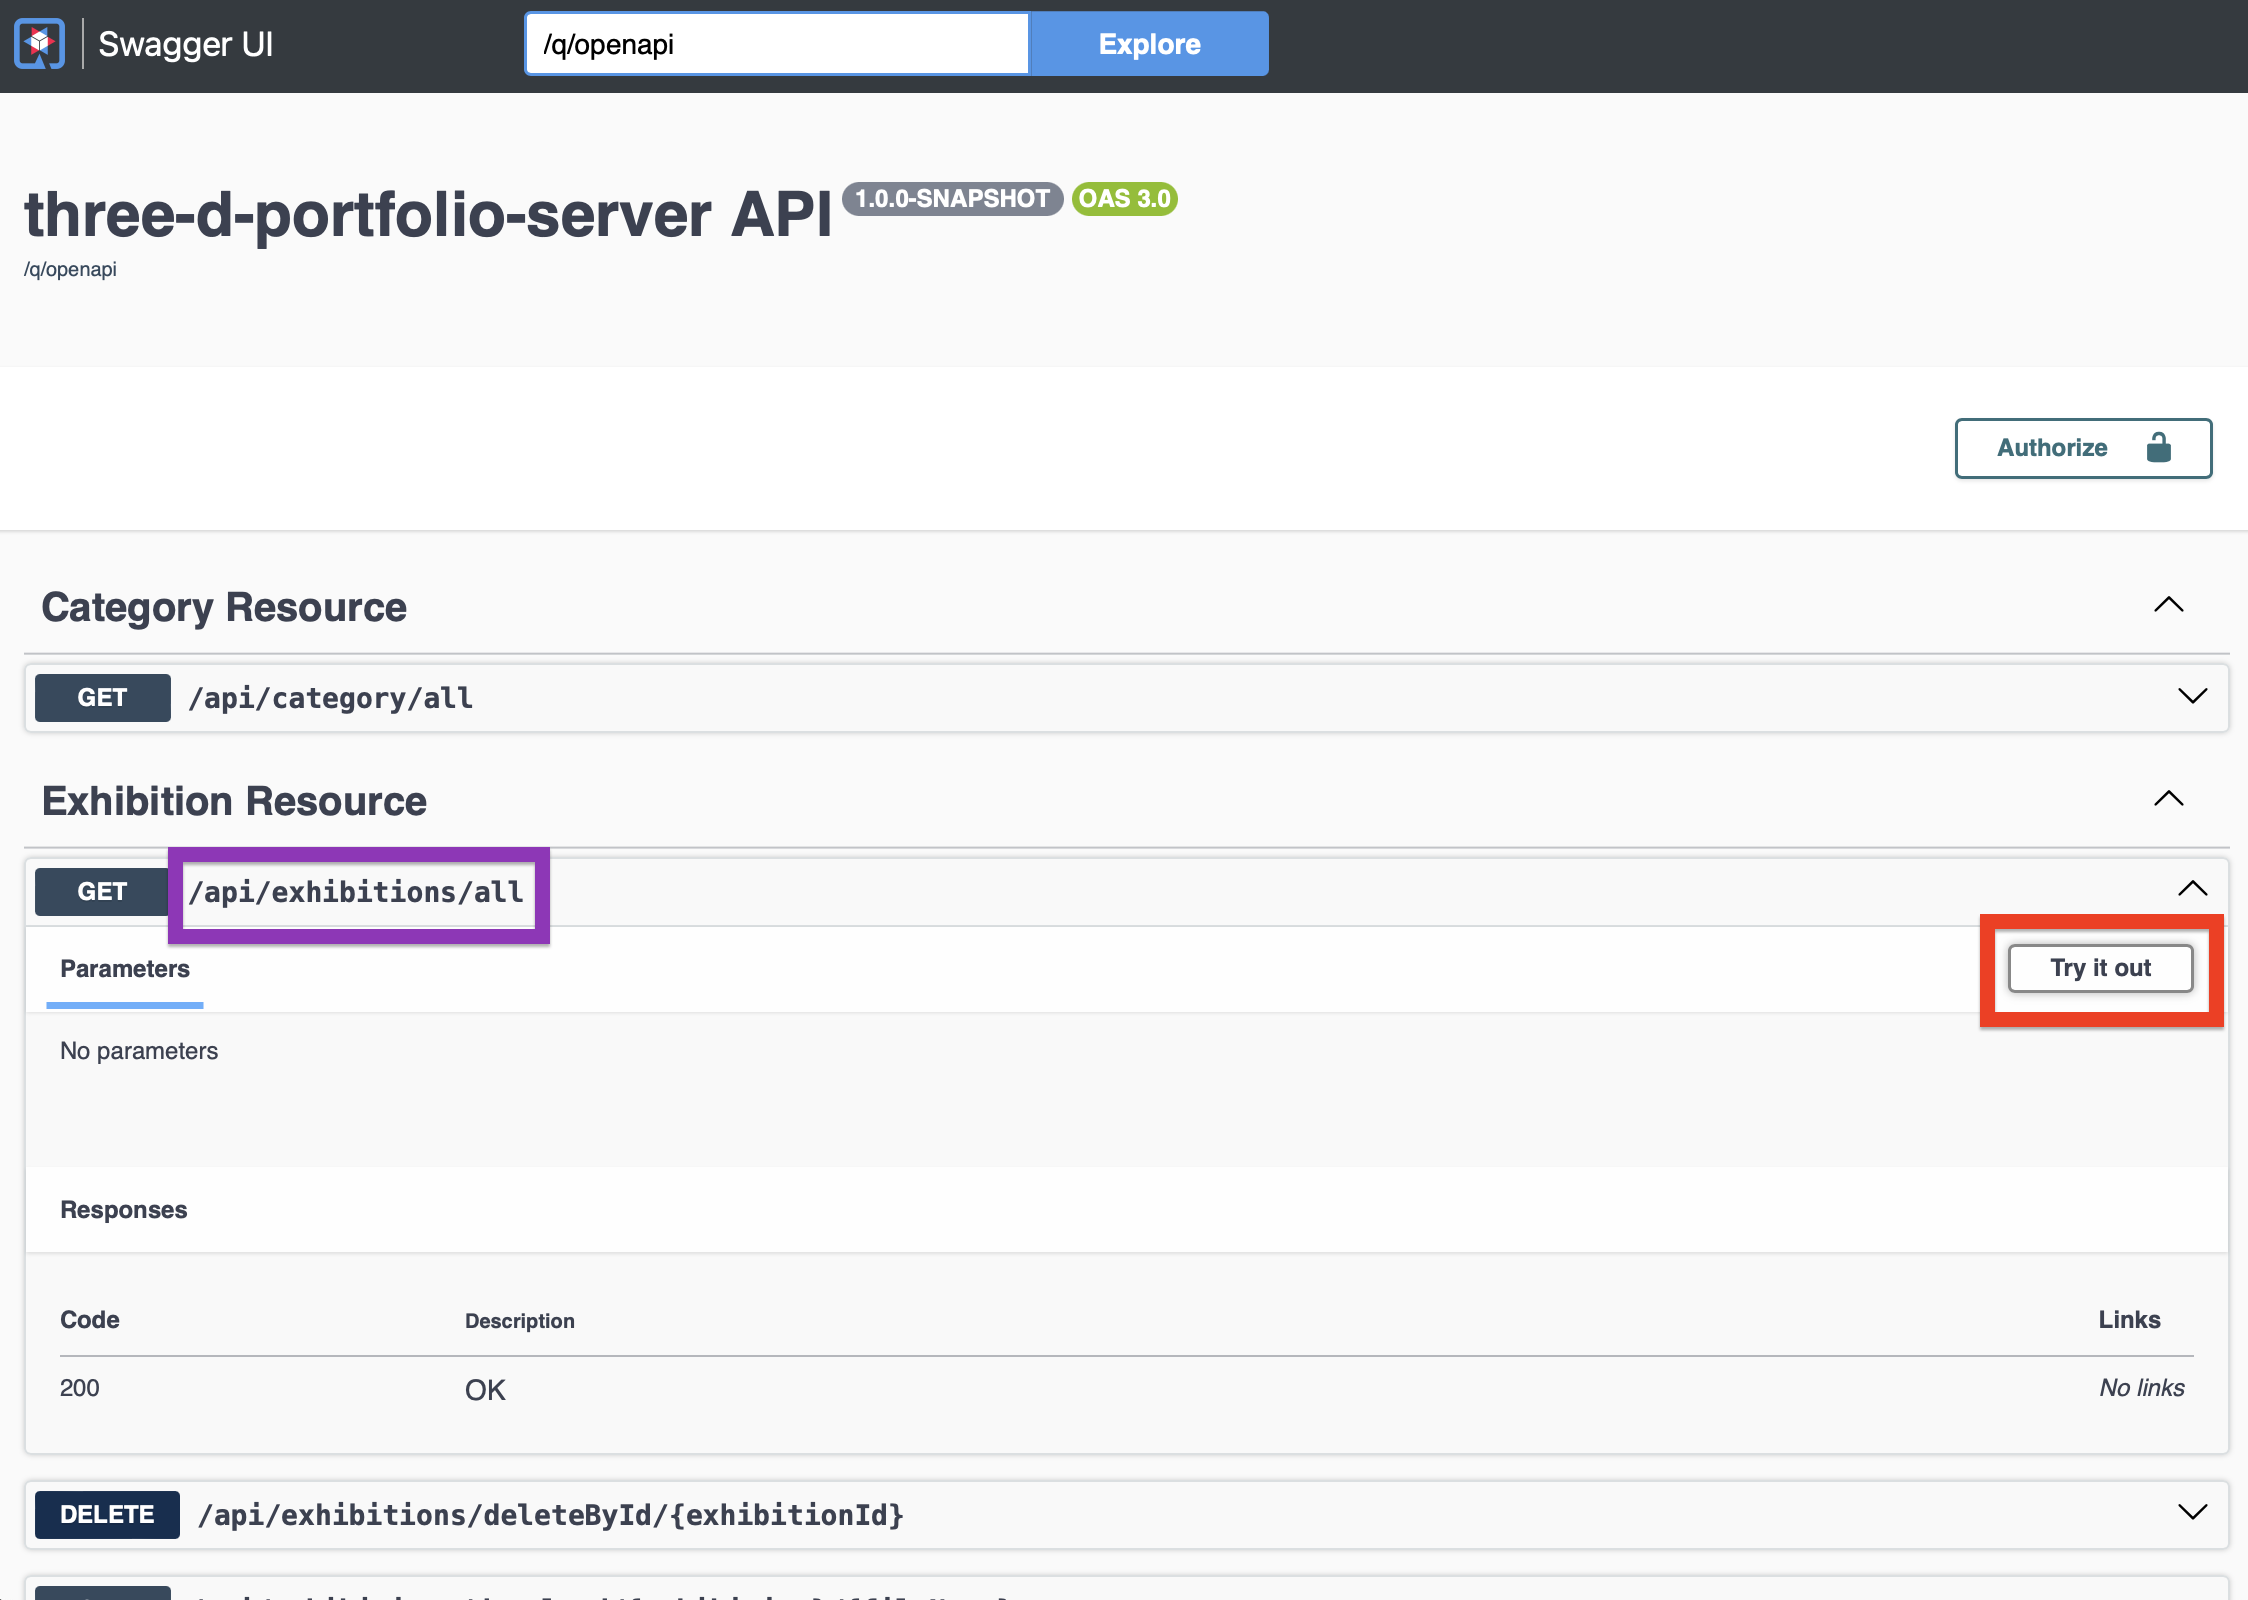
\includegraphics[scale=0.3]{pics/swaggerui.png}
    \caption{Übersicht der erstellten Schnittstellen}
    \label{fig:implementation:swaggerui}
\end{figure}

In Abbildung \ref{fig:implementation:swaggeruipost} lässt sich erkennen, dass die generierte Abfrage für numerische Werte standardmäßig \emph{0} und alphabetische Sequenzen \emph{string} einsetzt. 
Zweiteres ist kein Problem, da jedoch beim Anlegen jedes neuen Objekts die Id generiert wird, ist es einfacher, die Id aus dem Request zu entfernen. 
Falls jedoch ein bestimmter Wert für dieses Attribut gewünscht ist, muss die Einzigartigkeit der angelegten Entitäten beachtet werden. 
Ansonsten werden neue Objekt womöglich nicht gespeichert.

\begin{figure}
    \centering
    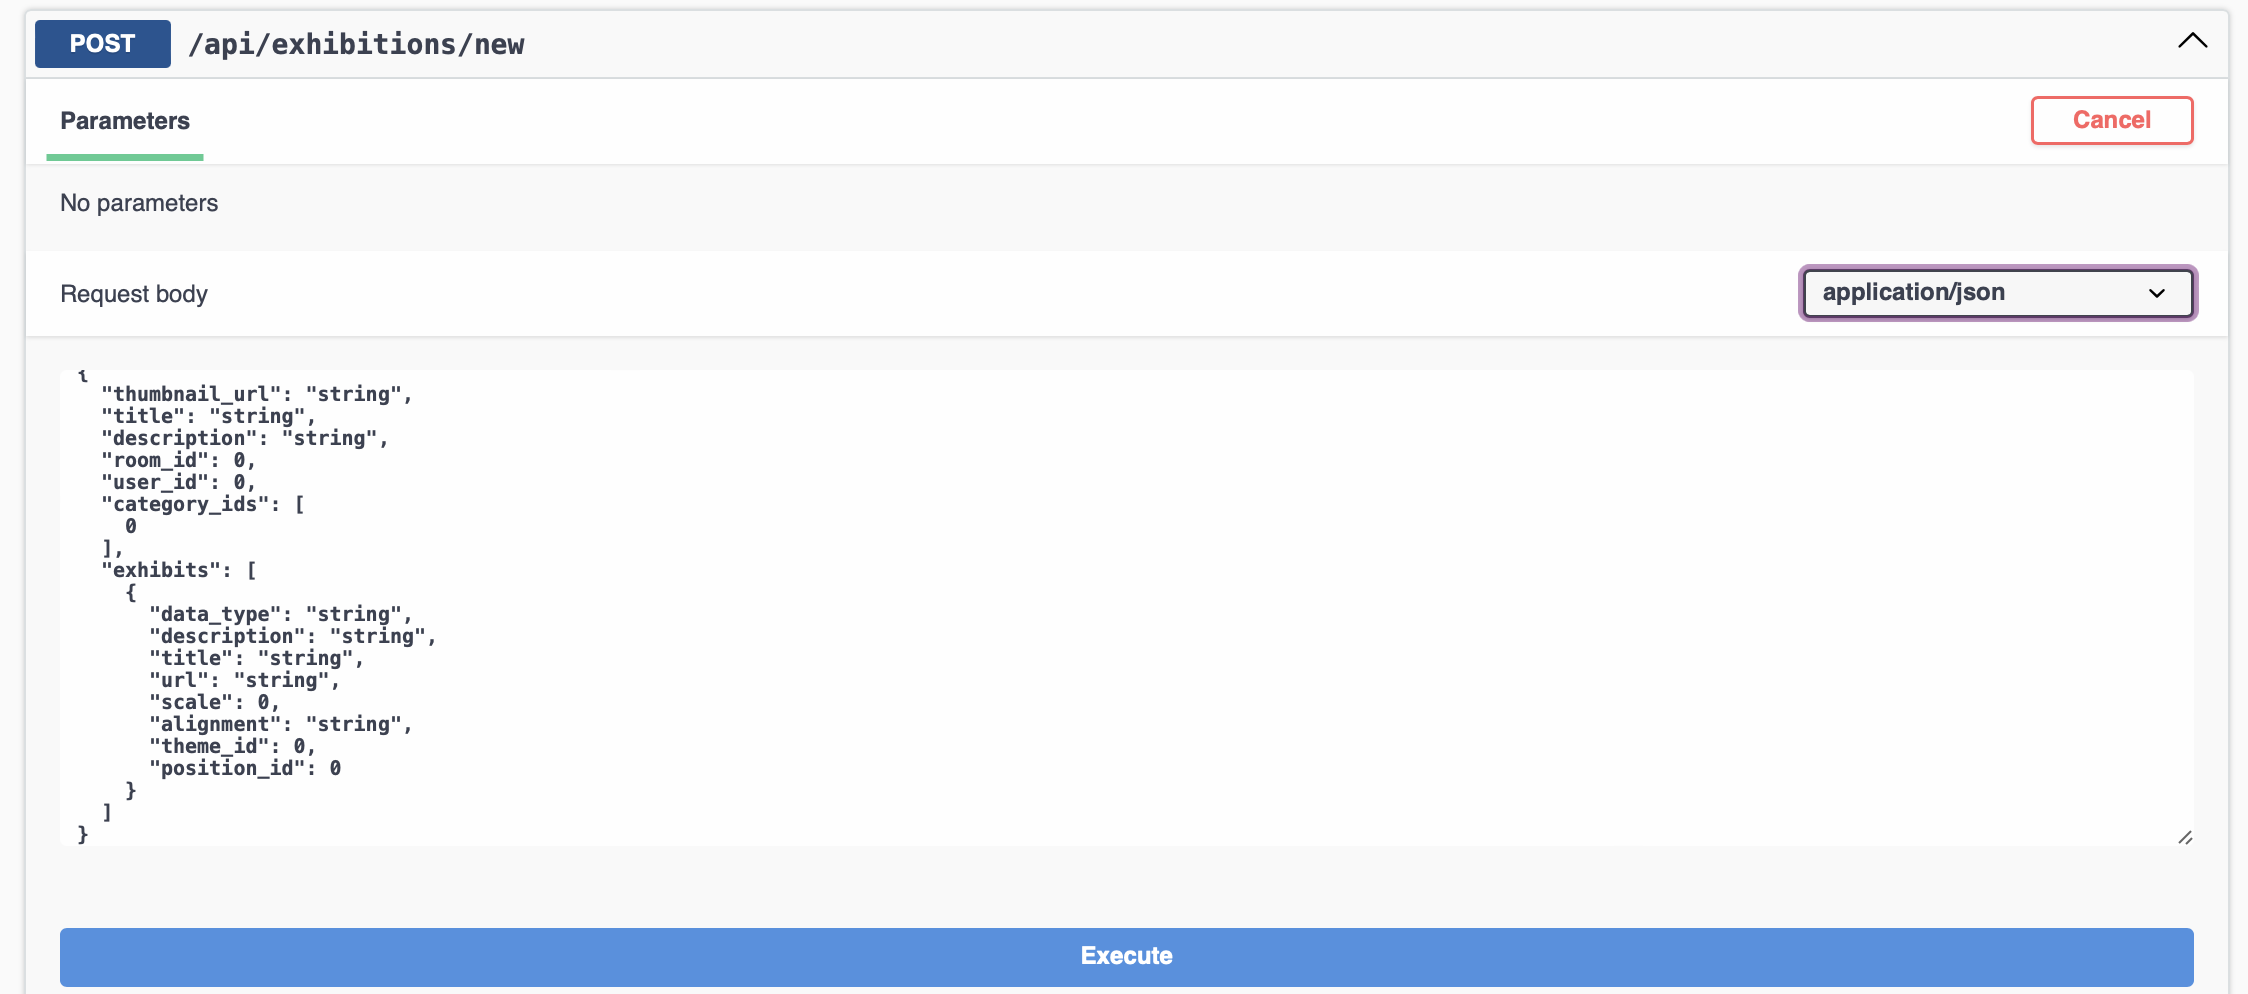
\includegraphics[scale=0.3]{pics/swaggeruipost.png}
    \caption{Automatisch generierte JSON-Anfrage}
    \label{fig:implementation:swaggeruipost}
\end{figure}

\subsection{Nach der Entwicklung}
Tests sind eine gute Möglichkeit, zu gewährleisten, dass die Applikation fehlerfrei ihre Aufgaben erledigt. 
Diese müssen eine breite Auswahl von möglichen Situationen abdecken.

In dieser Arbeit wird mit JUnit 5 und Mockito gearbeitet. 
Mockito ermöglicht es, die Repositories zu rekonstruieren. 
\cite{quarkusMockAbout}
\begin{lstlisting}[label=JUnit 5 Abhängigkeit in pom.xml, language=xml]
<dependency>
    <groupId>io.quarkus</groupId>
    <artifactId>quarkus-junit5-mockito</artifactId>
    <scope>test</scope>
</dependency>
\end{lstlisting}

Tests in Quarkus werden mit \emph{@QuarkusTest} gekennzeichnet. 
Mocks werden durch \emph{@InjectMock} erstellt.
Diese stellen alle Methoden aus den gemockten Repositories zur Verfügung.
Zusätzlich besteht die Möglichkeit zu definieren, dass eine Methode vor jedem Test ausgeführt werden soll mittels \emph{@BeforeEach}. 
Die einzelnen Tests werden zusätzlich mit \emph{@Test} annotiert. 
\cite{quarkusMockAbout}

Durch die Priorisierung des Testvorganges während der Entwicklung, wurden die zusätzlich angelegten Testklassen nur für die wichtigsten Endpoints genutzt. 
Dazu zählt beispielsweise die Entität Exhibition. 
Im unteren Beispiel wird ein Requst auf den Endpoint \emph{api/exhibits/} erstellt, wobei keine Exhibition vorhanden ist. 
Dadurch wird der Statuscode 404 erwartet. 
\begin{lstlisting}[label=Ein Exhibition Test, language=Java]
@Test
public void testGetExhibitByIncorrectId() {
    given()
            .when()
            .pathParam("exhibitionId", 1L)
            .get("/api/exhibitions/{exhibitionId}")
            .then()
            .statusCode(404);
}
\end{lstlisting}


\section{Hosten auf einer Cloud}

Bisher zu diesem Zeitpunkt musste die Applikation immer lokal ausgeführt werden. 
Dafür wurden auf jedem Gerät Java, Maven, PostgreSQL, Angular und der node package manager benötigt.


hei ;3


\section{Continious Integration und Deployment}

Zusätzlich war eine Implementation einer Continious Integration, sowie eines Continious Deployments geplant. 
Die beiden Begriffe lassen sich mit CI/CD abkürzen.
Sie sind für eine Automatisierung zuständig während der Softwareentwicklung. 

\subsection{Continious Integration}

Eine Continious Integration bedeutet, dass die Applikationsänderungen mittels mehrerer Überprüfungen auf ihre Funktionalität getestet wird.
Dies ist besonders praktikabel, wenn im Projekt mehrere Entwickler Änderungen im Code vornehmen. 
Eine CI-Pipeline stellt sicher, dass diese keinen Konflikt verursachen bei der Zusammenführung dieser verschiedener Versionen entsteht. 
Dies geschieht, durch Ausführung des Programms und eine Validierung der Tests. 
\cite{cicdabout}

Solch eine Automatisierung kann durch mehrere Arten verwirklicht werden, wie beispielsweise durch GitHub Actions. 
In jedem GitHub Repository gibt es eine Registerkarte namens \emph{Actions}, diese bietet Vorschläge zur Erstellung solch einer Pipeline (siehe Abb. \ref{fig:implementation:ghactions}). 

\begin{figure}
    \centering
    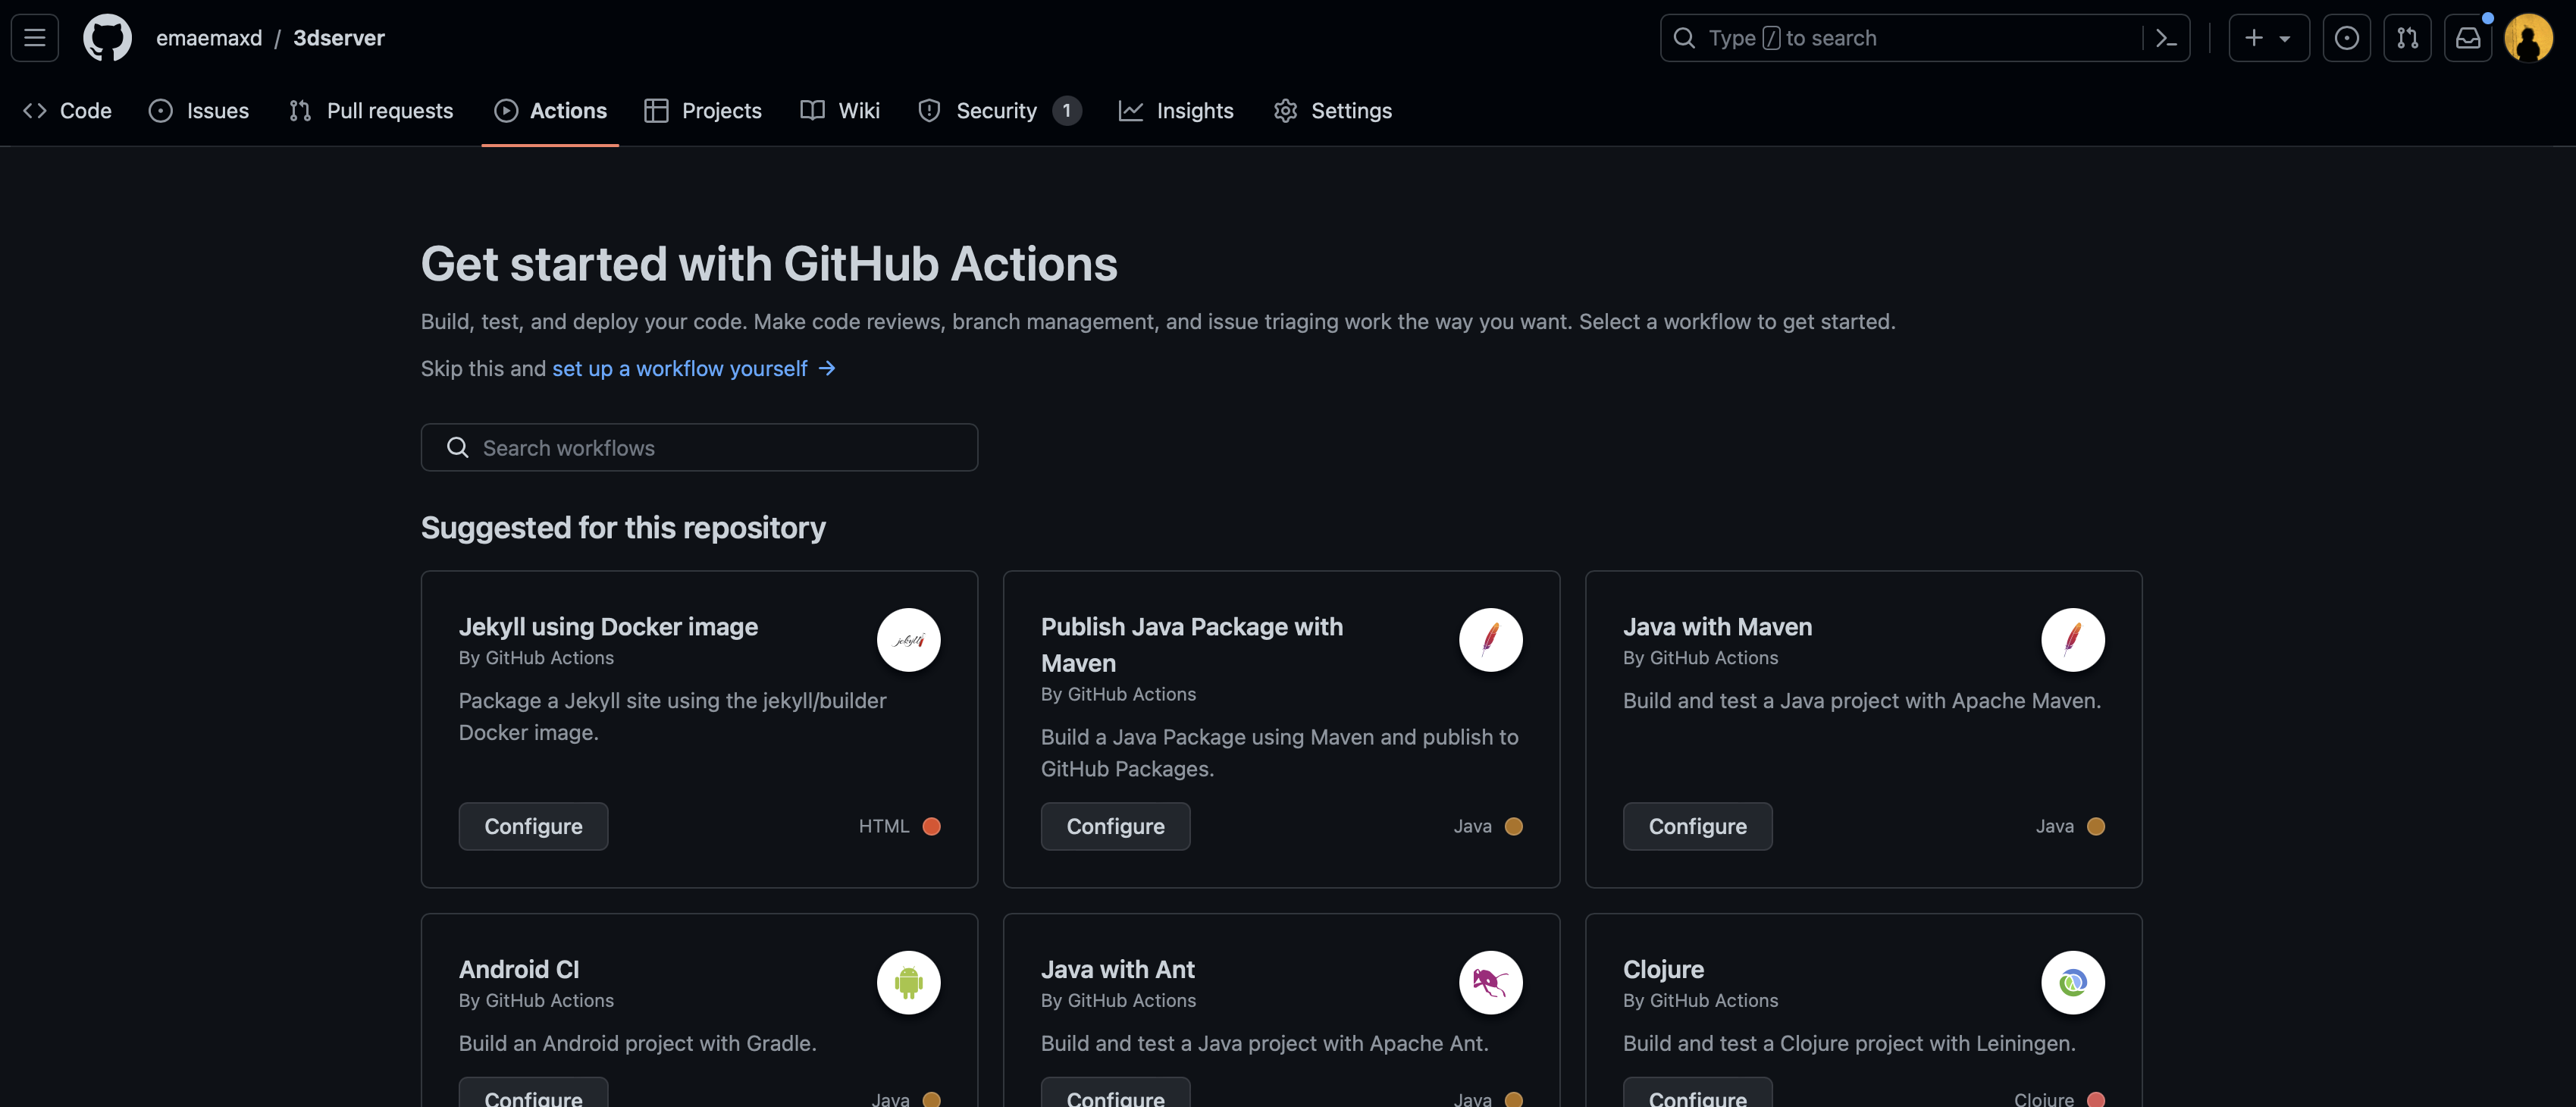
\includegraphics[scale=0.25]{pics/githubactions.png}
    \caption{GitHub Actions Benutzeroberfläche}
    \label{fig:implementation:ghactions}
\end{figure}

Jede Pipeline, oder auch Prozesskette, sind Dateien, welche in einem Ordner namens \emph{workflows} angelegt werden. 
In diesen Dateien sind Prozesse und Konfigurationen definiert, wie beispielsweise der Name der Pipeline.
Ebenso wird definiert, wann diese ausgeführt werden. 
Im Codeausschnitt \ref{lst:cipipeline} in Zeile 3 bis 7 wurde definiert, dass die nachfolgenden Steps bei jedem Push- und Pull-Request am Main Branch ausgeführt werden. 
Ebenso wird der benötigte Runner definiert in Zeile 11. 
Danach werden die einzelnen Schritte definiert, um die \gls{ci} für die Applikation zu erstellen, zum Beispiel die Installation aller node Module. 
In diesem Fall sind alle Steps Teil von einem einzigen Job namens "build". 

\begin{lstlisting}[label=lst:cipipeline, language=bash, caption=Pipeline einer CI]
name: CI

on:
  push:
    branches: [ main ]
  pull_request:
    branches: [ main ]
  # ...
jobs:
  build:
    runs-on: ubuntu-latest

    steps:
      - uses: actions/checkout@v2

      - name: Install all node modules
        run: npm i 
        working-directory: ./3D-Portfolio-Gallery/
    # ...

\end{lstlisting}

\subsection{Continious Delivery}

Eine \gls{cd} ist sozusagen der ein Upgrade der \gls{ci}. 
Das Ziel dieser ist es, die Applikation für die Produktion bereitzustellen. 
Dies geschieht ebenfalls durch eine Pipeline, welche die Anwendung Schritt für Schritt durchtestet und anschließend auf den Produktionsserver lädt. 
\cite{cicdabout}

In diesem Projekt wäre die Pipeline für die Ausführung der \emph{build.sh}-Datei zuständig gewesen. 
Zusätzlich hätte die Entfernung der Pods definiert werden müssen. 

Während der Entwicklung kam es zu dem Fazit, dass eine Konfiguration einer CI/CD Pipeline als nicht nötig empfunden wurde. 
Dies ist einerseits, da nur eine Person an dem Backend arbeitete und somit keine zweite Validierung der Software nötig war, da diese schon manuell ausgeführt wurden. 
Andererseits hätte es eine große Komplexität bedeutet, da Frontend und Backend auf unterschiedlichen Repositories entwickelt wurden und erst zum Schluss vereint. 
 
